% COMPOSITE

\subsection{Problem Set}

\subsubsection{(Problem 1) Conceptual Question 2.7}

The figure below shows the position--versus--time graph for a moving object.

\begin{center}
	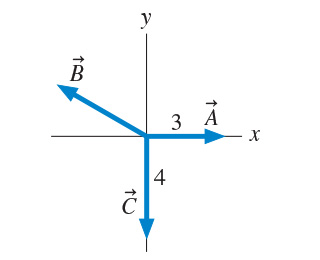
\includegraphics[width=0.5\textwidth]{"/Users/max/course-manager/data/semester/Spring 2025/course/PHY2111/chapter/Kinematics in One Dimension/section/2.1-2.7/figures/figure_1.png"}
\end{center}

\subsubsection{Part A}
At which numbered point or points is the object moving the fastest?

\begin{solution}
	Since the slope at a given point on an object's position--versus--time graph is it's velocity at that point, \fbox{numbered point 3} represents the fastest motion for the object.
\end{solution}

\subsubsection{Part B}
At which numbered point or points is the object moving to the left, if the positive $x$--direction corresponds to its rightward movement?

\begin{solution}
	\fbox{Point 6} corresponds to leftward movement since the slope is negative, given that the positive $x$--direction (up) corresponds to rightward movement.
\end{solution}

\subsubsection{Part C}
At which numbered point or points is the object speeding up?

\begin{solution}
	The object is speeding up at \fbox{points 2 and 6} since the absolute value of the slope is increasing.
\end{solution}

\subsubsection{Part D}
At which numbered point or points is the object turning around?

\begin{solution}
	The object is turning around at \fbox{point 5} because it represents a local extrema.
\end{solution}

\newpage

\subsubsection{(Problem 2) Conceptual Question 2.8}

The figure below shows six frames from the motion diagrams of two moving cars, $A$ and $B$.

\begin{center}
	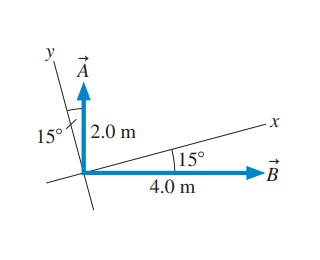
\includegraphics[width=0.5\textwidth]{/Users/max/course-manager/data/semester/Spring 2025/course/PHY2111/chapter/Kinematics in One Dimension/section/2.1-2.7/figures/figure_2.jpg
	}
\end{center}

\subsubsection{Part A}
Do the two cars ever have the same position at one instant of time?

\begin{solution}
	Yes, at \fbox{frames 3 and 6}.
\end{solution}

\subsubsection{Part C}
Do the two cars ever have the same velocity at one instant of time? If so, between which two frames?

\begin{solution}
	Yes, \fbox{between dots 4 and 5}. This is because car B is slowing down to (presumably) a stop, from a speed greater than car A. This means that at one instant the cars share the same velocity, and this instant must happen between dots 4 and 5.
\end{solution}

\newpage

\subsubsection{(Problem 3) Conceptual Question 2.11}

\subsubsection{Part A}
Select an example of a vertical motion with a positive velocity and a negative acceleration. Select the correct example and explanation.

\begin{solution}
	I chose the option "\textbf{A tossed ball on its way upward. As the ball moves upward it is slowing down, hence the acceleration is opposite the velocity (negative).}" This accurately describes an object with positive velocity and negative acceleration, assuming that the upwards direction represents positive velocity.
\end{solution}

\subsubsection{Part B}
Select an example of a vertical motion with a negative velocity and a negative acceleration. Select the correct example and explanation.

\begin{solution}
	I chose the option "\textbf{A tossed ball on its way down. As the ball moves down it is speeding up, hence the acceleration is pointing in the same direction as the velocity (negative).}" This accurately describes an object with negative velocity and negative acceleration, assuming that the upwards direction represents positive velocity.
\end{solution}

\newpage

\subsubsection{(Problem 4) Problem 2.2 -- Enhanced -- with Expanded Hints}
Julie drives \SI{100}{mi} to Grandmother's house. On the way to Grandmother's, Julie drives half the distance at \SI{40}{mph} and half the distance at \SI{60}{mph}. On her return trip, she drives half the time at \SI{40}{mph} and half the time at \SI{60}{mph}.

\subsubsection{Part A}
What is Julie's average speed on the way to Grandmother's house?
Express your answer with the appropriate units.

\begin{solution}
	\begin{align*}
		\frac{\SI{50}{miles}}{\SI{40}{mph}} &= \SI{1.25}{hr} \\
		\frac{\SI{50}{miles}}{\SI{60}{mph}} &= \SI{0.833}{hr} \\
		\SI{1.25}{hr} + \SI{0.833}{hr} &= \SI{2.0833}{hr} \\
		\frac{\SI{100}{miles}}{\SI{2.0833}{hr}} &= \boxed{\SI{48}{mph}} \\
	\end{align*}
\end{solution}

\subsubsection{Part B}
What is her average speed on the return trip?
Express your answer with the appropriate units.

\begin{solution}
	We can assume that Julie travels at \SI{40}{mph} for one hour and at \SI{60}{mph} for another hour, since $\SI{40}{miles} + \SI{60}{miles} = \SI{100}{miles}$. This means her trip time was \SI{2}{hours}. Therefore, her average speed was \fbox{\SI{50}{mph}}.
\end{solution}

\newpage

\subsubsection{(Problem 5) What $\mathbf{x}$ vs. $\mathbf{t}$ Graphs Can Tell You}

\begin{center}
	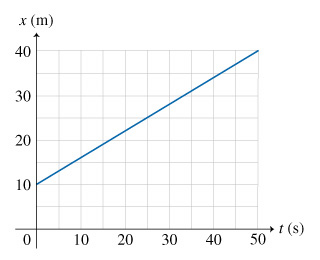
\includegraphics[width=0.5\textwidth]{/Users/max/course-manager/data/semester/Spring 2025/course/PHY2111/chapter/Kinematics in One Dimension/section/2.1-2.7/figures/figure_3.jpg
	}
\end{center}

\subsubsection{Part A}
What is the overall displacement $\Delta x$ of the particle? Express your answer in meters.

\begin{solution}
	Displacement is the distance from the starting point (after all motion is complete), therefore the displacement for the particle is
	\[
		\SI{40}{m}-\SI{10}{m}=\boxed{\SI{30}{m}}
	\]
\end{solution}

\subsubsection{Part B}
What is the average velocity $v_{\mathrm{av}}$ of the particle over the time interval $\Delta t=\SI{50}{s}$?
Express your answer in meters per second.

\begin{solution}
	The average velocity between two points on a position--versus--time graph is simply the slope between those points. Therefore,
	\begin{align*}
		v_{\mathrm{av}} &= \frac{y_2-y_1}{x_2-x_1} \\
		&= \frac{\SI{40}{m} - \SI{10}{m}}{\SI{50}{s}-\SI{0}{s}} \\
		&= \boxed{\SI{0.6}{\frac{m}{s}}} \\
	\end{align*}
\end{solution}

\subsubsection{Part C}
What is the instantaneous velocity $v$ of the particle at $t=\SI{10}{s}$?

\begin{solution}
	This graph is simple because the slope is constant, meaning the velocity is constant. Therefore, the answer above applies as well. However, more generally, the instantaneous velocity is the derivative of the pvt graph.
\end{solution}

\subsubsection{Part D}
Which of the graphs shown is the correct $v$ vs. $t$ plot for the motion described in the previous parts?

\begin{solution}
	I chose graph D, because it shows a constant velocity at $v=\SI{0.6}{\frac{m}{s}}$.
	\begin{center}
		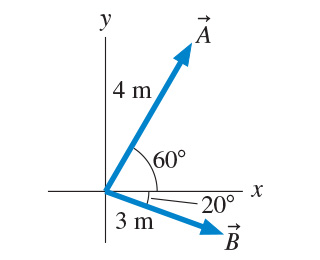
\includegraphics[width=0.5\textwidth]{/Users/max/course-manager/data/semester/Spring 2025/course/PHY2111/chapter/Kinematics in One Dimension/section/2.1-2.7/figures/figure_4.jpg
		}
	\end{center}
\end{solution}

\subsubsection{Part E}
Shown in the figure is the $v$ vs. $t$ curve selected in the previous part. What is the area $A$ of the shaded region under the curve?

\begin{center}
	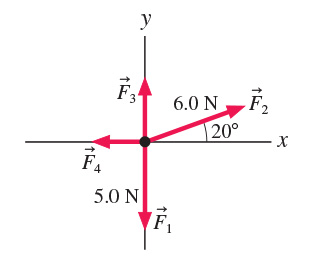
\includegraphics[width=0.5\textwidth]{/Users/max/course-manager/data/semester/Spring 2025/course/PHY2111/chapter/Kinematics in One Dimension/section/2.1-2.7/figures/figure_5.jpg
	}
\end{center}

\begin{solution}
	We can simply multiply the time by the velocity since it is constant, meaning that \fbox{$A=\SI{30}{m}$}. However, a more general approach would be with an integral, which I will demonstrate.
	\begin{align*}
		\int_{0}^{50} 0.6 \dt &= \left[ 0.6 \right]_{0}^{50} \\
		&= 0.6\left( 50 \right)-0.6\left( 0 \right) \\
		&= 30
	\end{align*}
\end{solution}

\newpage

\subsubsection{(Problem 6) Problem 2.10 -- Enhanced -- with Expanded Hints}

The figure below shows the velocity graph of a particle moving along the x-axis. Its initial position is $x_0 = \SI{2}{m}$ at $t_0 = \SI{0}{s}$.

\begin{center}
	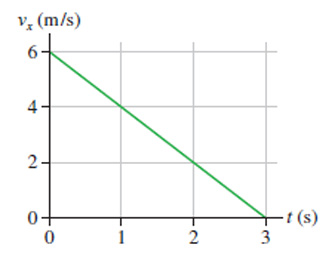
\includegraphics[width=0.5\textwidth]{/Users/max/course-manager/data/semester/Spring 2025/course/PHY2111/chapter/Kinematics in One Dimension/section/2.1-2.7/figures/figure_6.jpg
	}
\end{center}

\subsubsection{Part A}
At $t=\SI{1}{s}$, what is the particle's position?

\begin{solution}
	\begin{align*}
		v(t) &= -2x + 6 \\
		p(t) &= \int -2t + 6 \dt = -t^2 + 6t + C \\
		&= -t^2 + 6t + 2 \longleftarrow \text{given} \\
		p(1) &= -\left( 1 \right)^2 + 6\left( 1 \right) + 2 \\
		&= \boxed{\SI{7}{m}}
	\end{align*}
\end{solution}

\subsubsection{Part B}
At $t=\SI{1}{s}$, what is the particle's velocity?

\begin{solution}
	\begin{align*}
		v(t) &= -2x + 6 \\
		v(1) &= -2 + 6 \\
		&= \boxed{\SI{4}{\frac{m}{s}}}
	\end{align*}
\end{solution}

\subsubsection{Part C}
At $t=\SI{1}{s}$, what is the particle's acceleration?

\begin{solution}
	\begin{align*}
		v(t) &= -2x+6 \\
		a(t) &= v'(t) = \boxed{\SI{-2}{\frac{m}{s^2}}}
	\end{align*}
\end{solution}

\newpage

\subsubsection{(Problem 7) Clear the Runway}
To take off from the ground, an airplane must reach a sufficiently high speed. The velocity required for the takeoff, the takeoff velocity, depends on several factors, including the weight of the aircraft and the wind velocity.

\subsubsection{Part A}
A plane accelerates from rest at a constant rate of $\SI{5}{\frac{m}{s^2}}$ along a runway that is \SI{1800}{m} long. Assume that the plane reaches the required takeoff velocity at the end of the runway. What is the time $t_{\mathrm{takeoff}}$ needed to take off? Express your answer in seconds using three significant figures.

\begin{solution}
	\begin{align*}
		a(t) &= 5 \\
		v(t) &= \int 5 \dt = 5t + C = 5t ~ \text{(since $C$ is given as 0)} \\
		p(t) &= \int 5t = \frac{5}{2} t^2 + C = \frac{5}{2}t^2 \\
		& \text{(since the initial position $C$ is assumed as 0)}
	\end{align*}
	\begin{align*}
		1800 &= \frac{5}{2}t^2 \\
		\sqrt{\frac{3600}{5}} &= t \\
		\Aboxed{t &\approx \SI{26.8}{s}}
	\end{align*}
\end{solution}

\subsubsection{Part B}
What is the speed $v_{\mathrm{takeoff}}$ of the plane as it takes off? Express your answer numerically in meters per second using three significant figures.

\begin{solution}
	We found that
	\[
		v(t) = 5t
		.\]
	Therefore,
	\begin{align*}
		v(26.83) &= 5 \cdot 26.83 \approx \boxed{\SI{134}{\frac{m}{s}}}
	\end{align*}
\end{solution}

\subsubsection{Part C}
What is the distance $d_{\mathrm{first}}$ traveled by the plane in the first second of its run? Express your answer numerically in meters using three significant figures.

\begin{solution}
	\begin{align*}
		p(t) &= \frac{5}{2}t^2 \\
		d_{\mathrm{first}} &= p(1) - p(0) \\
		&= \frac{5}{2}\left( 1 \right)^2 - \frac{5}{2}\left( 0 \right)^2 \\
		&= \frac{5}{2} = \boxed{\SI{2.5}{m}} \\
	\end{align*}
\end{solution}

\subsubsection{Part D}
What is the distance $d_{\mathrm{last}}$ traveled by the plane in the last second before taking off? Express your answer numerically in meters  using three significant figures.

\begin{solution}
	\begin{align*}
		p(t) &= \frac{5}{2}t^2 \\
		d_{\mathrm{last}} &= p(\sqrt{720}) - p(\sqrt{720}-1) \\
		&= \frac{5}{2} \left( \sqrt{720} \right)^2 - \frac{5}{2} \left( \sqrt{720} -1 \right)^2 \\
		&\approx \boxed{\SI{132}{m}}
	\end{align*}
\end{solution}

\subsubsection{Part E}
What percentage of the takeoff velocity did the plane gain when it reached the midpoint of the runway? Express your answer numerically to the nearest percent.

\begin{solution}
	\begin{align*}
		v(t) &= 5t \\
	\end{align*}
	Midpoint time:
	\begin{align*}
		900 &= \frac{5}{2}t^2 \\
		t &= \sqrt{360} \\
	\end{align*}
	\begin{align*}
		v_{\mathrm{takeoff}} &= \sqrt{720} \\
		v_{\mathrm{midpoint}} &= \sqrt{360} \\
		\frac{\sqrt{360}}{\sqrt{720}} &= 0.7071067\ldots \approx \SI{71}{\percent} \\
	\end{align*}
\end{solution}

\newpage

\subsubsection{(Problem 8) Problem 2.17}
A speed skater moving to the left across frictionless ice at \SI{7.9}{m/s} hits a \SI{5}{m}-wide patch of rough ice. She slows steadily, then continues on at \SI{5.8}{m/s}.

\subsubsection{Part A}
What is the magnitude of her acceleration on the rough ice?

\begin{solution}
	\begin{align*}
		v_{\mathrm{initial}} &= \SI{-7.9}{\frac{m}{s}} \\
		v_{\mathrm{final}} &= \SI{-5.8}{\frac{m}{s}} \\
		d &= \SI{5}{m} \\
		v_{\mathrm{final}}^2 &= v_{\mathrm{initial}}^2 + 2ad \\
		a &= \frac{v_{\mathrm{final}}^2 - v_{\mathrm{initial}}^2}{2d} \\
		a &= \frac{-5.8^2- \left( -7.9^2 \right)}{10} \\
		a &= \frac{-33.64 - \left( -62.41^2 \right)}{10} \\
		a &= \frac{-33.64 - \left( -62.41 \right)}{10} \\
		&= \boxed{\SI{2.877}{\frac{m}{s^2}}}
	\end{align*}
\end{solution}

\newpage

\subsubsection{(Problem 9) PSS 2.1 Kinematics with Constant Acceleration}
A car is traveling at a constant velocity of magnitude $v_0$ when the driver notices a garbage can on the road in front of him. At that moment, the distance between the garbage can and the front of the car is $d$. A time $t_{\mathrm{react}}$ after noticing the garbage can, the driver applies the brakes and slows down at a constant rate before coming to a halt just before the garbage can. What is the magnitude of the car's acceleration after the brakes are applied?

\subsubsection{Part A}
Below is a sketch of the situation described in this problem, along with four different motion diagrams. Which of these diagrams is the correct pictorial representation of the problem?

\begin{center}
	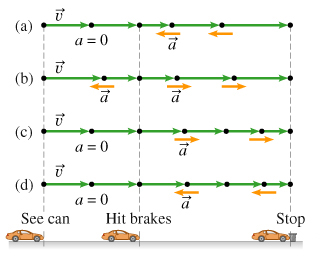
\includegraphics[width=0.5\textwidth]{/Users/max/course-manager/data/semester/Spring 2025/course/PHY2111/chapter/Kinematics in One Dimension/section/2.1-2.7/figures/figure_7.jpg
	}
\end{center}

\begin{solution}
	I chose diagram d because it show deceleration (an acceleration vector pointing in the opposite direction of motion).
\end{solution}

\subsubsection{Part B}
As an alternative to the pictorial representation shown above, you could consider using a graphical representation instead. Below are four velocity-versus-time graphs. Which graph correctly represents the situation described in this problem?

\begin{center}
	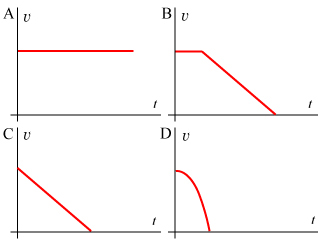
\includegraphics[width=0.5\textwidth]{/Users/max/course-manager/data/semester/Spring 2025/course/PHY2111/chapter/Kinematics in One Dimension/section/2.1-2.7/figures/figure_8.jpg
	}
\end{center}

\begin{solution}
	I chose graph B because it shows a reaction time.
\end{solution}

\subsubsection{Part C}
Find the magnitude of $a_x$, the acceleration of the car after the brakes are applied. Express your answer in terms of some or all of the variables $d$, $t_{\mathrm{react}}$, and $v_0$.

\begin{solution}
	\begin{align*}
		d_{\mathrm{react}} &= v_0 \cdot t_{\mathrm{react}} \\
		d_{\mathrm{brake}} &= d-d_{\mathrm{react}} \\
		&= d-v_0 \cdot t_{\mathrm{react}} \\
		v_{f}^2 &= v_{i}^2 + 2a_{x}d_{\mathrm{brake}} \\
		0 &= v_0^2 + 2a_{x}d_{\mathrm{brake}} \\
		a_{x} &= \abs{ - \frac{v_0^2}{2 \left( d-v_0 \cdot t_{\mathrm{react}} \right)} }  \\
		a_{x} &= \frac{v_0^2}{2 \left( d-v_0 \cdot t_{\mathrm{react}} \right)} \\
	\end{align*}
\end{solution}

\subsubsection{Part D}
Based on [the expression from part C], what happens to $\abs{ a_{x} }$ if $t_{\mathrm{react}}$ increases and all the other variables remain constant?

\begin{solution}
	I chose the option "\textbf{$\abs{ a_x }$ increases because it is inversely proportional to a linear function of because it is inversely proportional to a linear function of  $t_{\mathrm{react}}$ that decreases as  $t_{\mathrm{react}}$ increases. that decreases as $t_{\mathrm{react}}$ increases.}" because it correctly describes the relationship between $t_{\mathrm{react}}$ and $a_{x}$.
\end{solution}

\newpage

\subsubsection{(Problem 10) Problem 2.15}
It has been proposed that a very small probe could be sent to a nearby star system by using a powerful laser beam, fired from an earth-orbiting satellite, to push on a lightweight "solar sail." Very high speeds could be reached in the vacuum of space by a fairly modest acceleration that continues for a long interval of time.

\subsubsection{Part A}
Write an expression for the constant acceleration $a_x$ an object needs to reach velocity $v_{\mathrm{max}}$ in time $t_{\mathrm{push}}$, starting from rest.

\begin{solution}
	\begin{align*}
		a_x &= \frac{v_{\mathrm{max}}}{t_{\mathrm{push}}}
	\end{align*}
\end{solution}

\subsubsection{Part B}
Write an expression in terms of $v_{\mathrm{max}}$ and $t_{\mathrm{push}}$ for the distance $d$ the object travels during this time.

\begin{solution}
	\begin{align*}
		d &= \frac{1}{2} v_{\mathrm{max}} t_{\mathrm{push}}
	\end{align*}
\end{solution}

\subsubsection{Part C}
For the mission to be feasible, the probe needs to reach 10\% of the speed of light after being pushed for 1.0 year. The probe would then coast the rest of the way. What constant acceleration is needed?

\begin{solution}
	\begin{align*}
		v_{\mathrm{max}} &= 0.1c = \SI{3.00e7}{m/s} \\
		t_{\mathrm{push}} &= \SI{3.156e7}{s} \\
		a_x &= \frac{\SI{3.00e7}{m/s}}{\SI{3.156e7}{s}} = \SI{0.951}{m/s^2}
	\end{align*}
\end{solution}

\subsubsection{Part D}
What fraction of a light year will the probe have traveled at the end of the year? A light year (ly) is the distance traveled by light in 1 year.

\begin{solution}
	\begin{align*}
		d &= \frac{1}{2} v_{\mathrm{max}} t_{\mathrm{push}} \\
		&= \frac{1}{2} \cdot \SI{3.00e7}{m/s} \cdot \SI{3.156e7}{s} = \SI{4.74e14}{m} \\
		1 \, \mathrm{ly} &= \SI{9.461e15}{m} \\
		\frac{d}{1 \, \mathrm{ly}} &= \frac{\SI{4.74e14}{m}}{\SI{9.461e15}{m}} \approx \SI{5.01}{\percent}
	\end{align*}
\end{solution}

\newpage

\subsubsection{(Problem 11) A Flea in Flight}
In this problem, you will apply kinematic equations to a jumping flea. Take the magnitude of free-fall acceleration to be \SI{9.80}{m/s^2}. Ignore air resistance.

A flea jumps straight up to a maximum height of \SI{0.430}{m}. What is its initial velocity $v_0$ as it leaves the ground?

Express your answer in meters per second to three significant figures.

\begin{solution}
	\begin{align*}
		v_f^2 &= v_0^2 + 2a \Delta y \\
		0 &= v_0^2 - 2 \cdot \SI{9.80}{m/s^2} \cdot \SI{0.430}{m} \\
		v_0 &= \sqrt{2 \cdot \SI{9.80}{m/s^2} \cdot \SI{0.430}{m}} \\
		v_0 &= \SI{2.90}{m/s}
	\end{align*}
\end{solution}

\subsubsection{Part B}
How long is the flea in the air from the time it jumps to the time it hits the ground?

Express your answer in seconds to three significant figures.

\begin{solution}
	\begin{align*}
		t &= \frac{2v_0}{g} \\
		t &= \frac{2 \cdot \SI{2.90}{m/s}}{\SI{9.80}{m/s^2}} \\
		t &= \SI{0.592}{s}
	\end{align*}
\end{solution}

\newpage

\subsubsection{(Problem 12) Problem 2.36 -- Enhanced -- with Hints and Feedback}

The position of a particle is given by the function $x = (4t^3 - 9t^2 + 12) \, \mathrm{m}$, where \( t \) is in seconds.

\subsubsection{Part A}
At what time does the particle reach its minimum velocity?

Express your answer with the appropriate units.

\begin{solution}
	\begin{align*}
		v(t) &= \frac{dx}{dt} = 12t^2 - 18t \\
		\frac{dv}{dt} &= a(t) = 24t - 18 \\
		0 &= 24t - 18 \\
		t &= \frac{18}{24} = \SI{0.75}{s}
	\end{align*}
\end{solution}

\subsubsection{Part B}
What is \( (v_x)_{\mathrm{min}} \)?

Express your answer with the appropriate units.

\begin{solution}
	\begin{align*}
		v(0.75) &= 12(0.75)^2 - 18(0.75) \\
		&= 12(0.5625) - 13.5 \\
		&= 6.75 - 13.5 \\
		&= \SI{-6.75}{m/s}
	\end{align*}
\end{solution}

\subsubsection{Part C}
At what time is the acceleration zero?

Express your answer with the appropriate units.

\begin{solution}
	\begin{align*}
		a(t) &= 24t - 18 \\
		0 &= 24t - 18 \\
		t &= \frac{18}{24} = \SI{0.75}{s}
	\end{align*}
\end{solution}

\newpage

\subsubsection{(Problem 13) Problem 2.40 -- Enhanced -- with Hints and Feedback}

A particle's velocity is described by the function \( v_x = k t^2 \), where \( v_x \) is in \( \mathrm{m/s} \), \( t \) is in \( \mathrm{s} \), and \( k \) is a constant. The particle's position at \( t_0 = 0 \, \mathrm{s} \) is \( x_0 = -5.60 \, \mathrm{m} \). At \( t_1 = 2.00 \, \mathrm{s} \), the particle is at \( x_1 = 5.10 \, \mathrm{m} \).

\subsubsection{Part A}
Determine the units of \( k \) in terms of \( \mathrm{m} \) and \( \mathrm{s} \).

\begin{solution}
	Given \( v_x = k t^2 \), the units of \( v_x \) are \( \mathrm{m/s} \) and \( t \) is in \( \mathrm{s} \).
	\begin{align*}
		[v_x] &= [k] [t^2] \\
		\mathrm{m/s} &= [k] \cdot \mathrm{s^2} \\
		[k] &= \frac{\mathrm{m/s}}{\mathrm{s^2}} \\
		[k] &= \mathrm{m/s^3}
	\end{align*}
\end{solution}

\subsubsection{Part B}
Determine the value of the constant \( k \).

Express your answer in meters per second.

\begin{solution}
	The position \( x(t) \) is obtained by integrating \( v_x = k t^2 \):
	\begin{align*}
		x(t) &= \int v_x \, dt = \int k t^2 \, dt \\
		&= \frac{k t^3}{3} + C
	\end{align*}

	Using the initial condition \( x(0) = -5.60 \, \mathrm{m} \), we find \( C = -5.60 \, \mathrm{m} \).

	At \( t = 2.00 \, \mathrm{s} \):
	\begin{align*}
		5.10 &= \frac{k (2.00)^3}{3} - 5.60 \\
		5.10 + 5.60 &= \frac{8k}{3} \\
		10.70 &= \frac{8k}{3} \\
		k &= \frac{10.70 \times 3}{8} \\
		k &= \SI{4.01}{m/s^3}
	\end{align*}
\end{solution}

\newpage

\subsubsection{(Problem 14) Problem 2.41}

A particle's acceleration is described by the function \( a_x = (10 - t) \, \mathrm{m/s^2} \), where \( t \) is in seconds. Its initial conditions are \( x_0 = 190 \, \mathrm{m} \) and \( v_{0x} = 0 \, \mathrm{m/s} \) at \( t = 0 \, \mathrm{s} \).

\subsubsection{Part A}
At what time is the velocity again zero?

Express your answer with the appropriate units.

\begin{solution}
	The velocity is found by integrating the acceleration:
	\begin{align*}
		v(t) &= \int (10 - t) \, dt = 10t - \frac{1}{2} t^2 + C
	\end{align*}

	Using the initial condition \( v(0) = 0 \), we find \( C = 0 \). To find when the velocity is zero again:
	\begin{align*}
		0 &= 10t - \frac{1}{2} t^2 \\
		t \left(10 - \frac{1}{2} t \right) &= 0 \\
		t &= 0 \quad \text{or} \quad t = 20 \, \mathrm{s}
	\end{align*}

	The velocity is zero again at \( \boxed{\SI{20}{s}} \).
\end{solution}

\subsubsection{Part B}
What is the particle's position at that time?

Express your answer with the appropriate units.

\begin{solution}
	The position is found by integrating the velocity:
	\begin{align*}
		x(t) &= \int \left(10t - \frac{1}{2} t^2 \right) dt \\
		&= 5t^2 - \frac{1}{6} t^3 + C
	\end{align*}

	Using the initial condition \( x(0) = 190 \, \mathrm{m} \), we find \( C = 190 \).

	At \( t = 20 \, \mathrm{s} \):
	\begin{align*}
		x(20) &= 5(20)^2 - \frac{1}{6} (20)^3 + 190 \\
		&= 5(400) - \frac{1}{6}(8000) + 190 \\
		&= 2000 - 1333.33 + 190 \\
		&= \SI{856.67}{m}
	\end{align*}

	The particle's position at that time is \( \boxed{\SI{856.67}{m}} \).
\end{solution}

\newpage

\subsubsection{(Problem 15) Problem 2.47 -- Enhanced -- with Expanded Hints}

You are driving to the grocery store at \( 20 \, \mathrm{m/s} \). You are \( 130 \, \mathrm{m} \) from an intersection when the traffic light turns red. Assume that your reaction time is \( 0.50 \, \mathrm{s} \) and that your car brakes with constant acceleration.

\subsubsection{Part A}
What magnitude braking acceleration will bring you to a stop exactly at the intersection?

Express your answer with the appropriate units.

\begin{solution}
	First, calculate the distance traveled during the reaction time:
	\begin{align*}
		d_{\mathrm{reaction}} &= v_0 \cdot t_{\mathrm{reaction}} \\
		&= 20 \cdot 0.50 \\
		&= \SI{10}{m}
	\end{align*}

	The remaining distance for braking is:
	\begin{align*}
		d_{\mathrm{braking}} &= 130 - 10 = \SI{120}{m}
	\end{align*}

	Using the kinematic equation:
	\begin{align*}
		v_f^2 &= v_0^2 + 2ad \\
		0 &= 20^2 + 2a(120) \\
		a &= -\frac{400}{240} \\
		a &= -\SI{1.67}{m/s^2}
	\end{align*}

	The magnitude of the braking acceleration is \( \boxed{\SI{1.67}{m/s^2}} \).
\end{solution}

\newpage

\subsubsection{(Problem 16) Problem 2.49 -- Enhanced -- with Hints and Feedback}

You're driving down the highway late one night at \( 20 \, \mathrm{m/s} \) when a deer steps onto the road \( 35 \, \mathrm{m} \) in front of you. Your reaction time before stepping on the brakes is \( 0.50 \, \mathrm{s} \), and the maximum deceleration of your car is \( 10 \, \mathrm{m/s^2} \).

\subsubsection{Part A}
How much distance is between you and the deer when you come to a stop?

Express your answer with the appropriate units.

\begin{solution}
	Distance traveled during the reaction time:
	\begin{align*}
		d_{\mathrm{reaction}} &= v_0 \cdot t_{\mathrm{reaction}} \\
		&= 20 \cdot 0.50 \\
		&= \SI{10}{m}
	\end{align*}

	Remaining distance for braking:
	\begin{align*}
		d_{\mathrm{braking}} &= \frac{v_0^2}{2a} \\
		&= \frac{20^2}{2 \cdot 10} \\
		&= \SI{20}{m}
	\end{align*}

	Total stopping distance:
	\begin{align*}
		d_{\mathrm{total}} &= d_{\mathrm{reaction}} + d_{\mathrm{braking}} \\
		&= 10 + 20 \\
		&= \SI{30}{m}
	\end{align*}

	Distance between you and the deer when you stop:
	\begin{align*}
		d_{\mathrm{deer}} &= 35 - 30 = \boxed{\SI{5}{m}}
	\end{align*}
\end{solution}

\subsubsection{Part B}
What is the maximum speed you could have and still not hit the deer?

Express your answer with the appropriate units.

\begin{solution}
	Let \( v_{\mathrm{max}} \) be the maximum speed. The total stopping distance should equal \( 35 \, \mathrm{m} \):
	\begin{align*}
		d_{\mathrm{reaction}} + d_{\mathrm{braking}} &= 35 \\
		v_{\mathrm{max}} \cdot 0.5 + \frac{v_{\mathrm{max}}^2}{2 \cdot 10} &= 35 \\
		0.5 v_{\mathrm{max}} + 0.05 v_{\mathrm{max}}^2 &= 35
	\end{align*}

	Rearranging into a quadratic equation:
	\begin{align*}
		0.05 v_{\mathrm{max}}^2 + 0.5 v_{\mathrm{max}} - 35 &= 0
	\end{align*}

	Solving for \( v_{\mathrm{max}} \):
	\begin{align*}
		v_{\mathrm{max}} &= \frac{ -0.5 \pm \sqrt{(0.5)^2 - 4(0.05)(-35)} }{2 \cdot 0.05} \\
		&= \frac{ -0.5 \pm \sqrt{0.25 + 7} }{0.1} \\
		&= \frac{ -0.5 \pm \sqrt{7.25} }{0.1} \\
		&= \frac{ -0.5 \pm 2.6926 }{0.1}
	\end{align*}

	Taking the positive root:
	\begin{align*}
		v_{\mathrm{max}} &\approx \frac{2.1926}{0.1} = \boxed{\SI{21.9}{m/s}}
	\end{align*}
\end{solution}

\newpage

\subsubsection{(Problem 17) Problem 2.56}

A \( 200 \, \mathrm{kg} \) weather rocket is loaded with \( 100 \, \mathrm{kg} \) of fuel and fired straight up. It accelerates upward at \( 35 \, \mathrm{m/s^2} \) for \( 32 \, \mathrm{s} \), then runs out of fuel. Ignore any air resistance effects.

\subsubsection{Part A}
What is the rocket's maximum altitude?

Express your answer with the appropriate units.

\begin{solution}
	First, calculate the velocity at burnout:

	\begin{align*}
		v_{\mathrm{burnout}} &= a t \\
		&= 35 \cdot 32 \\
		&= \SI{1120}{m/s}
	\end{align*}

	The distance covered during powered flight:

	\begin{align*}
		d_{\mathrm{powered}} &= \frac{1}{2} a t^2 \\
		&= \frac{1}{2} \cdot 35 \cdot 32^2 \\
		&= \SI{17920}{m}
	\end{align*}

	After burnout, the rocket will coast to its maximum height. Using:

	\begin{align*}
		v_f^2 &= v_i^2 + 2 a d \\
		0 &= 1120^2 - 2 \cdot 9.8 \cdot d_{\mathrm{coast}} \\
		d_{\mathrm{coast}} &= \frac{1120^2}{2 \cdot 9.8} \\
		&= \SI{64000}{m}
	\end{align*}

	Total maximum altitude:

	\begin{align*}
		h_{\mathrm{max}} &= d_{\mathrm{powered}} + d_{\mathrm{coast}} \\
		&= 17920 + 64000 \\
		&= \boxed{\SI{81920}{m}}
	\end{align*}
\end{solution}

\subsubsection{Part B}
How long is the rocket in the air before hitting the ground?

Express your answer with the appropriate units.

\begin{solution}
	Time to reach maximum height after burnout:

	\begin{align*}
		t_{\mathrm{coast}} &= \frac{v_i}{g} \\
		&= \frac{1120}{9.8} \\
		&= \SI{114.29}{s}
	\end{align*}

	Total time to reach maximum altitude:

	\begin{align*}
		t_{\mathrm{up}} &= 32 + 114.29 = \SI{146.29}{s}
	\end{align*}

	Time to fall back to the ground:

	\begin{align*}
		d &= \frac{1}{2} g t^2 \\
		81920 &= \frac{1}{2} \cdot 9.8 \cdot t^2 \\
		t &= \sqrt{\frac{2 \cdot 81920}{9.8}} \\
		&= \SI{129.3}{s}
	\end{align*}

	Total time in the air:

	\begin{align*}
		t_{\mathrm{total}} &= t_{\mathrm{up}} + t_{\mathrm{fall}} \\
		&= 146.29 + 129.3 \\
		&= \boxed{\SI{275.59}{s}}
	\end{align*}
\end{solution}

\newpage

\subsubsection{(Problem 18) Problem 2.57}

A lead ball is dropped into a lake from a diving board \( 5.40 \, \mathrm{m} \) above the water. After entering the water, it sinks to the bottom with a constant velocity equal to the velocity with which it hit the water. The ball reaches the bottom \( 3.00 \, \mathrm{s} \) after it is released.

\subsubsection{Part A}
How deep is the lake?

Express your answer with the appropriate units.

\begin{solution}
	First, find the time it takes to fall from the diving board to the water surface:

	\begin{align*}
		d &= \frac{1}{2} g t^2 \\
		5.40 &= \frac{1}{2} \cdot 9.8 \cdot t^2 \\
		t &= \sqrt{\frac{2 \cdot 5.40}{9.8}} \\
		t &= \SI{1.05}{s}
	\end{align*}

	Next, find the velocity upon hitting the water:

	\begin{align*}
		v &= g t \\
		&= 9.8 \cdot 1.05 \\
		&= \SI{10.29}{m/s}
	\end{align*}

	The time spent sinking:

	\begin{align*}
		t_{\mathrm{sinking}} &= 3.00 - 1.05 = \SI{1.95}{s}
	\end{align*}

	Now, calculate the depth of the lake:

	\begin{align*}
		d_{\mathrm{lake}} &= v \cdot t_{\mathrm{sinking}} \\
		&= 10.29 \cdot 1.95 \\
		&= \boxed{\SI{20.06}{m}}
	\end{align*}
\end{solution}

\newpage

\subsubsection{(Problem 19) Problem 2.25 -- Enhanced -- with Hints and Feedback}

A rock is dropped from the top of a tall building. The rock's displacement in the \emph{last second} before it hits the ground is 48\% of the \emph{entire distance} it falls.

\subsubsection{Part A}
How tall is the building?

Express your answer with the appropriate units.

\begin{solution}
	The total distance fallen in time \( T \) is:

	\begin{align*}
		D &= \frac{1}{2} g T^2
	\end{align*}

	The distance fallen in the last second:

	\begin{align*}
		d_{\mathrm{last}} &= \frac{1}{2} g T^2 - \frac{1}{2} g (T - 1)^2 \\
		&= \frac{1}{2} g \left( T^2 - (T^2 - 2T + 1) \right) \\
		&= \frac{1}{2} g (2T - 1)
	\end{align*}

	Given:

	\begin{align*}
		d_{\mathrm{last}} &= 0.48 D \\
		\frac{1}{2} g (2T - 1) &= 0.48 \cdot \frac{1}{2} g T^2 \\
		2T - 1 &= 0.48 T^2 \\
		0.48 T^2 - 2T + 1 &= 0
	\end{align*}

	Solving the quadratic equation:

	\begin{align*}
		T &= \frac{2 \pm \sqrt{4 - 1.92}}{0.96} \\
		&= \frac{2 \pm \sqrt{2.08}}{0.96} \\
		&\approx \frac{2 \pm 1.442}{0.96}
	\end{align*}

	Taking the positive root:

	\begin{align*}
		T &\approx \frac{2 + 1.442}{0.96} \\
		&\approx \SI{3.59}{s}
	\end{align*}

	Now, the total distance:

	\begin{align*}
		D &= \frac{1}{2} g T^2 \\
		&= \frac{1}{2} \cdot 9.8 \cdot (3.59)^2 \\
		&\approx \boxed{\SI{63.2}{m}}
	\end{align*}
\end{solution}

\newpage

\subsubsection{(Problem 20) Problem 2.68}

David is driving a steady \(\SI{24.0}{m/s}\) when he passes Tina, who is sitting in her car at rest. At the instant David passes her, Tina begins to accelerate at a steady \(\SI{2.10}{m/s^2}\).

\subsubsection{Part A}
How far does Tina drive before passing David?

Express your answer with the appropriate units.

\begin{solution}
	Let \( t \) be the time from when David passes Tina until she catches up.

	\begin{align*}
		\text{David's position (relative to start)} &:\quad x_D = (\SI{24.0}{m/s})\,t \\
		\text{Tina's position (relative to start)} &:\quad x_T = \frac{1}{2}(\SI{2.10}{m/s^2})\,t^2 = 1.05\,t^2.
	\end{align*}

	They meet when \( x_D = x_T \):

	\begin{align*}
		24.0\,t &= 1.05\,t^2 \\
		1.05\,t^2 - 24.0\,t &= 0 \\
		t\,(1.05t - 24.0) &= 0.
	\end{align*}

	Since \( t = 0 \) is the instant David passes Tina, the nontrivial solution is:

	\begin{align*}
		t &= \frac{24.0}{1.05} \approx \SI{22.857}{s}.
	\end{align*}

	The distance Tina travels before passing David is \( x_T \) at this \( t \):

	\begin{align*}
		x_T &= 1.05\,(22.857)^2 \approx \SI{549}{m}.
	\end{align*}
\end{solution}

\subsubsection{Part B}
What is her speed as she passes him?

Express your answer with the appropriate units.

\begin{solution}
	Tina starts from rest and accelerates at \( \SI{2.10}{m/s^2} \). At \( t \approx \SI{22.857}{s} \):

	\begin{align*}
		v_T &= (\SI{2.10}{m/s^2})\,t \approx 2.10 \times 22.857 \approx \SI{48.0}{m/s}.
	\end{align*}
\end{solution}

\newpage

\subsubsection{(Problem 21) Problem 2.73 -- Enhanced -- with Hints and Feedback}

When a 1984 Alfa Romeo Spider sports car accelerates at the maximum possible rate, its motion during the first 20 s is modeled by
\[
	v_x^2 = \frac{2P}{m} \cdot t,\quad\text{where}\quad P = 3.6 \times 10^4\,\mathrm{W},\; m = 1200\,\mathrm{kg},\; t\,\text{is in s},\; v_x\,\text{is in m/s}.
\]

\subsubsection{Part A}
Find an algebraic expression for the car's acceleration at time \( t \).
Express your answer in terms of some or all of the variables \( P \), \( m \), and \( t \).

\begin{solution}
	From \( v_x^2 = \tfrac{2P}{m} t\), we have
	\[
		v_x(t) = \sqrt{\frac{2P}{m} \, t}.
	\]
	The acceleration is \( a(t) = \frac{dv_x}{dt} \). Thus,
	\begin{align*}
		a(t) &= \frac{d}{dt}\Bigl(\sqrt{\tfrac{2P}{m}\,t}\Bigr)
		= \frac{1}{2}\,\sqrt{\frac{2P}{m}}\,t^{-1/2}
		= \boxed{\frac{1}{2}\sqrt{\frac{2P}{m}}\,\frac{1}{\sqrt{t}}}.\\
	\end{align*}
\end{solution}

\subsubsection{Part B}
What is the car's speed at \( t = \SI{2.0}{s}\)?

Express your answer with the appropriate units.

\begin{solution}
	Using \( v_x = \sqrt{\tfrac{2P}{m}\,t}\), with \( P = 3.6\times10^4\,\mathrm{W} \), \( m = 1200\,\mathrm{kg} \), and \( t = 2.0\,\mathrm{s}\):
	\begin{align*}
		v_x^2 &= \left(\frac{2\times3.6\times10^4}{1200}\right) (2.0) = 60 \times 2.0 = 120,\\
		v_x &= \sqrt{120} \approx \SI{10.95}{m/s} \approx \boxed{\SI{11.0}{m/s}}.\\
	\end{align*}
\end{solution}

\subsubsection{Part C}
What is the car's speed at \( t = \SI{10}{s}\)?

Express your answer with the appropriate units.

\begin{solution}
	Again using \( v_x = \sqrt{\tfrac{2P}{m}\,t}\) with \( t = 10\,\mathrm{s}\):
	\begin{align*}
		v_x^2 &= 60 \times 10 = 600,\\
		v_x &= \sqrt{600} \approx \SI{24.5}{m/s}.\\
	\end{align*}
\end{solution}

\subsubsection{Part D}
Evaluate the acceleration at \( t = \SI{2.0}{s}\).

Express your answer with the appropriate units.

\begin{solution}
	From \( a(t) = \frac{1}{2}\sqrt{\frac{2P}{m}}\,\frac{1}{\sqrt{t}} \) and \( \tfrac{2P}{m}=60\):
	\begin{align*}
		a(2.0) &= \frac{1}{2}\sqrt{60}\,\frac{1}{\sqrt{2}} \approx 3.873\times\frac{1}{1.414} \approx \SI{2.74}{m/s^2}.\\
	\end{align*}
\end{solution}

\subsubsection{Part E}
Evaluate the acceleration at \( t = \SI{10}{s}\).

Express your answer with the appropriate units.

\begin{solution}
	\begin{align*}
		a(10) &= 3.873\times\frac{1}{\sqrt{10}} \approx \frac{3.873}{3.162} \approx \SI{1.23}{m/s^2}.
	\end{align*}
\end{solution}

\newpage


\subsubsection{(Problem 22) Problem 2.80 -- Enhanced -- with Expanded Hints}

A rocket is launched straight up with constant acceleration. Four seconds after liftoff, a bolt falls off the side of the rocket. The bolt hits the ground \(6.20\,\mathrm{s}\) later.

\subsubsection{Part A}
What was the rocket's acceleration?

Express your answer with the appropriate units.

\begin{solution}
Let \(a\) be the rocket's constant acceleration, \(g=\SI{9.8}{m/s^2}\), \(t_1=\SI{4.0}{s}\) (liftoff to bolt release), and \(t_2=\SI{6.20}{s}\) (bolt release to ground).
\[
    v_{\mathrm{det}} = a\,t_1,\quad y_{\mathrm{det}} = \tfrac12\,a\,t_1^2.
\]
After detach:
\[
    0 = y_{\mathrm{det}} + v_{\mathrm{det}}\,t_2 - \tfrac12\,g\,t_2^2.
\]
Substitute \(t_1=4\), \(t_2=6.20\):
\begin{align*}
    0 &= \tfrac12 a(4)^2 + a(4)(6.20) - \tfrac12\,(9.8)(6.20)^2,\\
    0 &= 8a + 24.8a - 4.9\,(6.20)^2,\\
    32.8a &= 4.9\times38.44,\\
    a &\approx \frac{188.416}{32.8} = \SI{5.74}{m/s^2}.
\end{align*}
\end{solution}

